\begin{figure}[h!]

    
    
      \tikzstyle{latent} = [circle,fill=white,draw=black,inner sep=1pt,
minimum size=30pt, font=\fontsize{15}{15}\selectfont, node distance=1]


  \newcommand{\ltkiz}{1cm}
  
  
\captionsetup[subfigure]{justification=centering}
    \centering  
    \begin{subfigure}[t]{0.3\textwidth}
        \centering   
		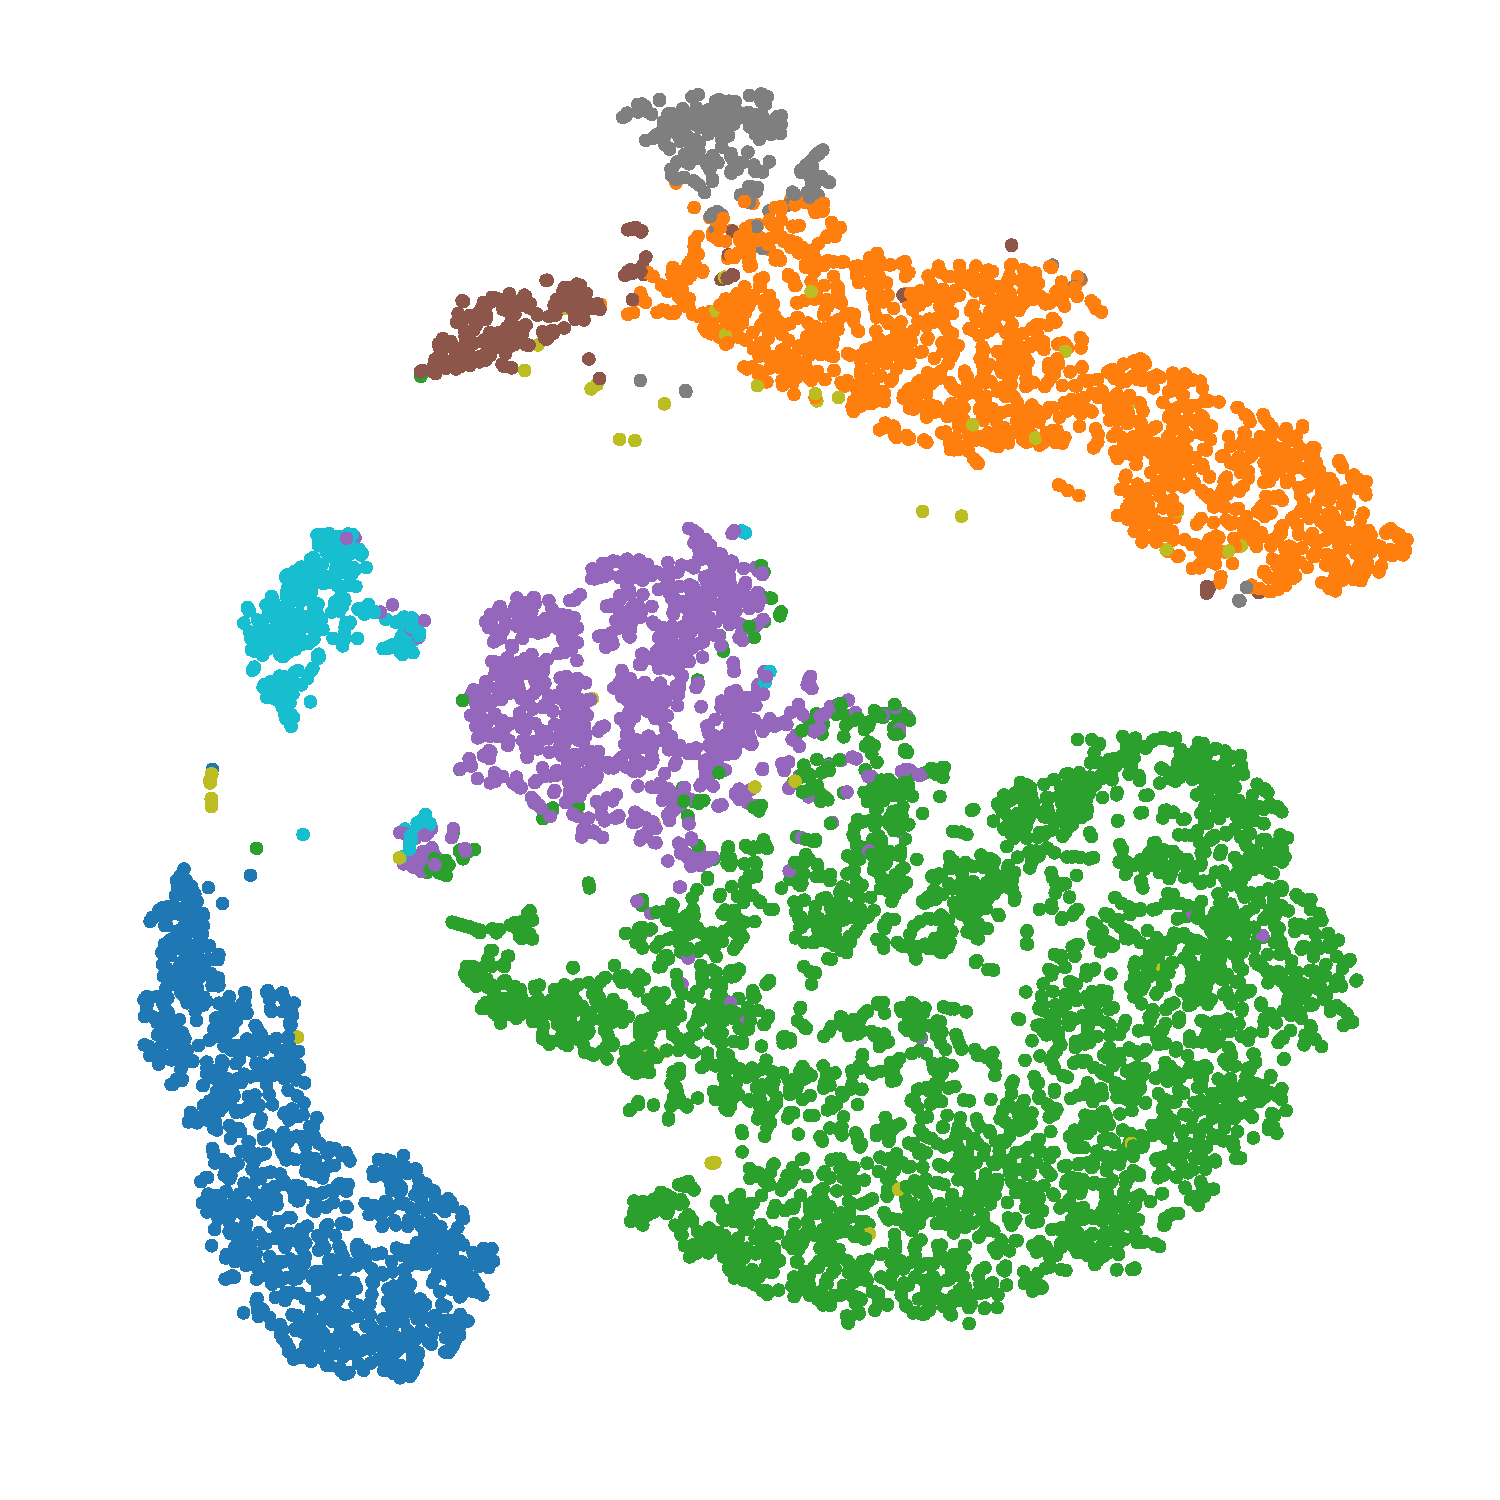
\includegraphics[width=3.5cm]{figures/cell_types.pdf}
        \caption{Embedding of $x$: gene expression data. Each point is a cell. Colors are cell-types.}
    \end{subfigure}%
    ~  
    \begin{subfigure}[t]{0.3\textwidth}
        \centering  
		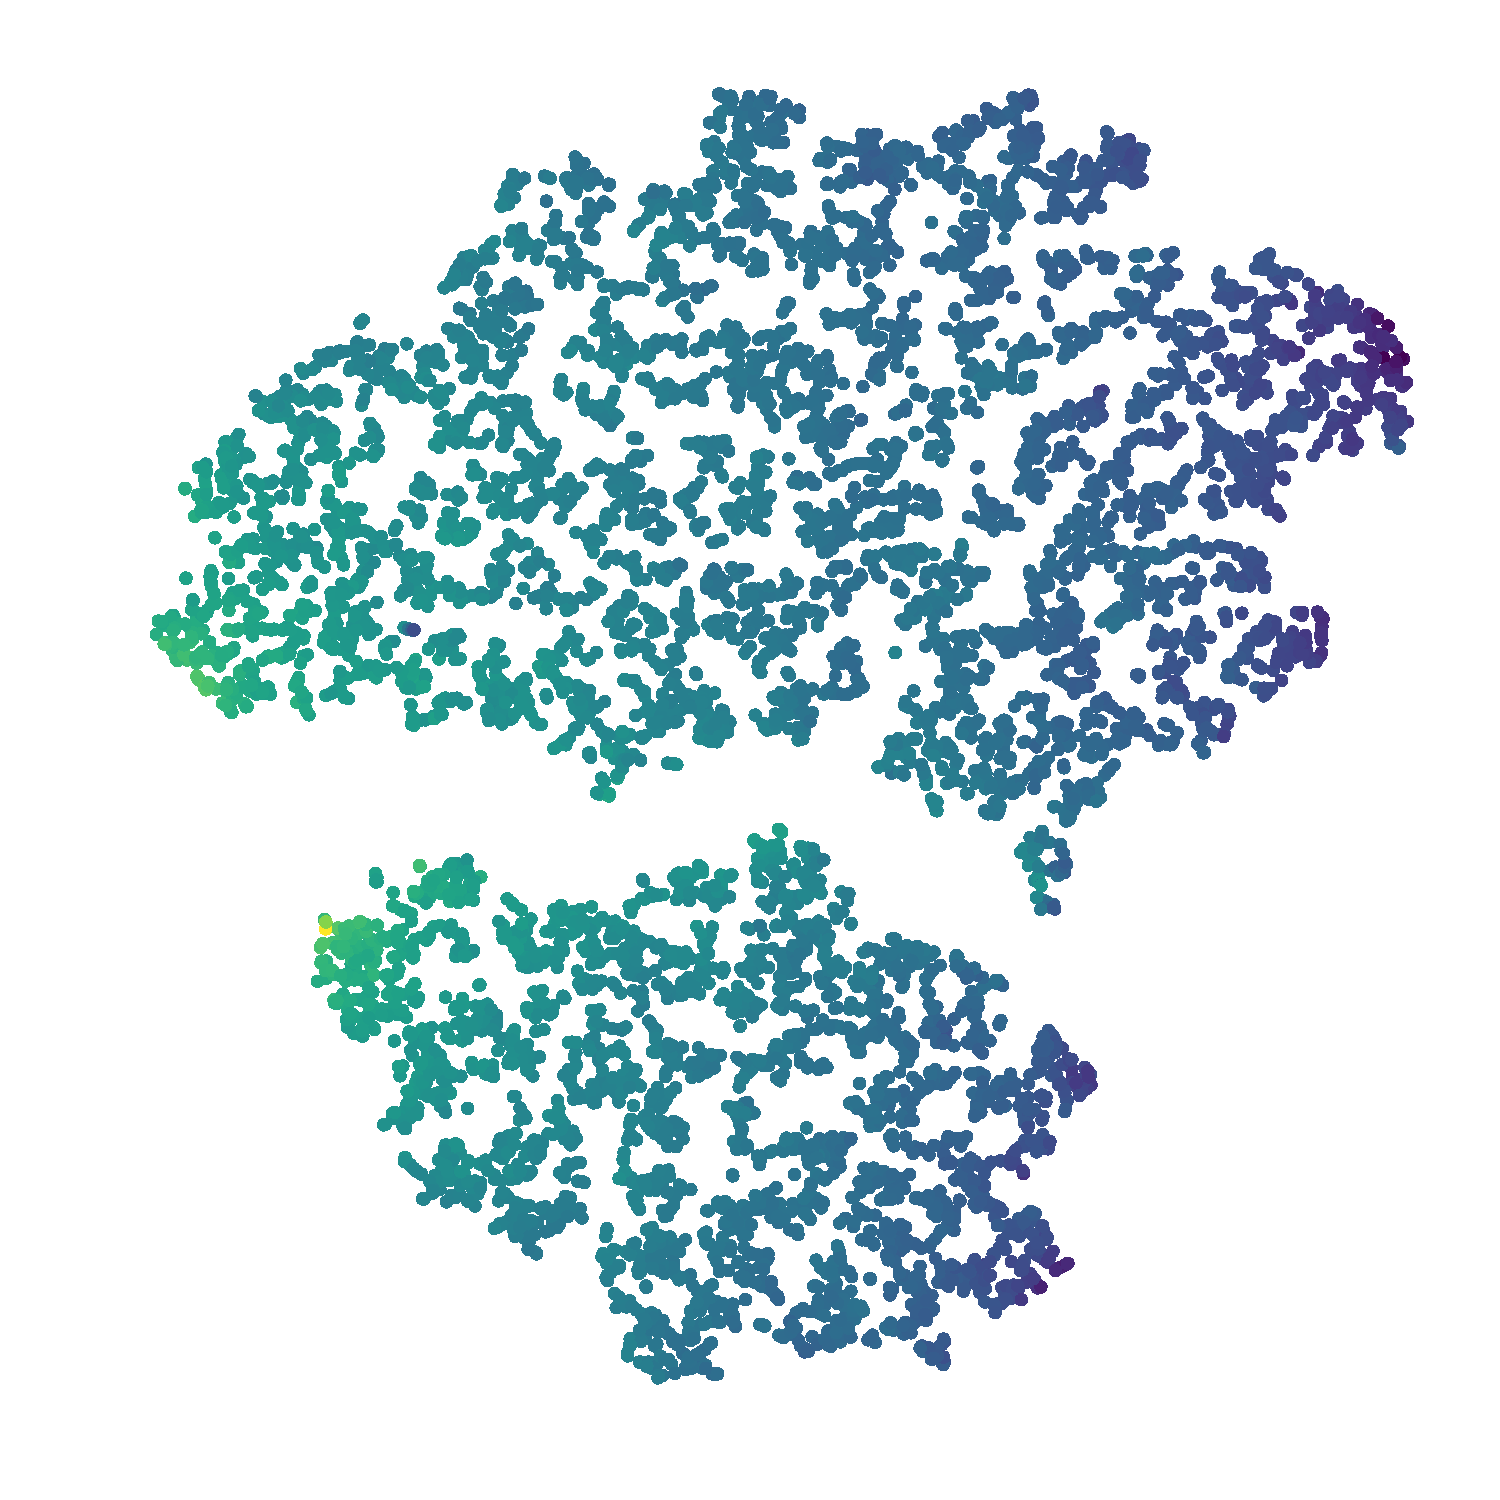
\includegraphics[width=0.7\textwidth]{figures/qc.pdf}
        \caption{Embedding of $s$: alignment errors. Each point is a cell. Color is $s^1$.}
    \end{subfigure}
    ~
    \begin{subfigure}[t]{0.3\textwidth}
        \centering  
		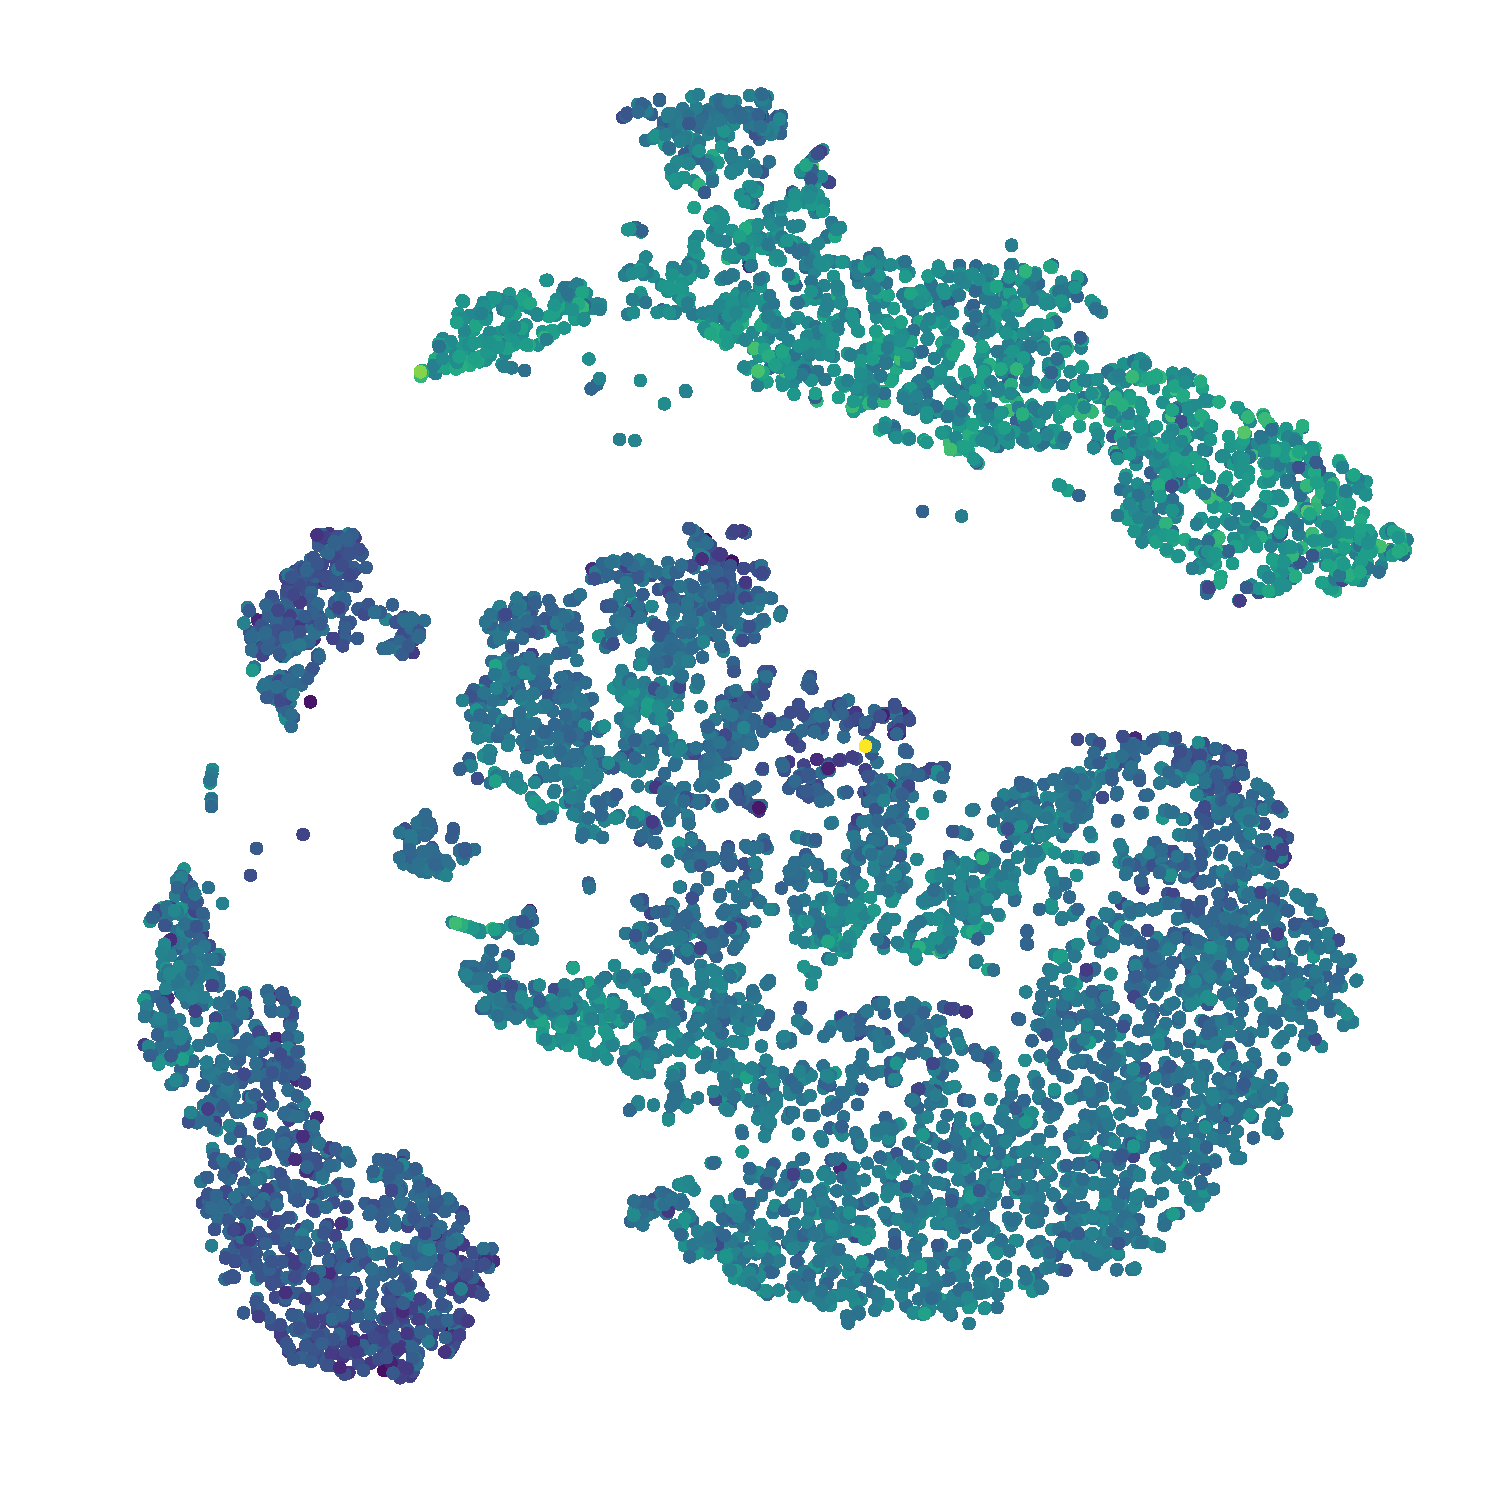
\includegraphics[width=0.7\textwidth]{figures/qc_5.pdf}
        \caption{Embedding of $x$: gene expression data. Each point is a cell. Color is the same quality control metric $s^1$.}
    \end{subfigure}

        \caption[Raw data from the PBMC dataset]{Raw data from the PBMC dataset. $s^1$ is the proportion of transcripts which confidently mapped to a gene for each cell.}
    \label{hsicpbmc}
\end{figure}